\section{Separable Similarity and Emissions}
\label{sec:separ-simil-emiss}

In the HDP-HMM-LT model, we have a defined set of states with 
locations $\ell_j$, $j = 1, \dots,
J$.  In Chapter \ref{chapter:cocktail-party}, the similarities depended on the same parameters that determined the emission distributions, which was denoted by $\theta_j$.  In Chapter \ref{chapter:cocktail-party},
each $\theta_j$ was a binary state vector, and the similarity $\phi_{jj'}$ was a decreasing function of the distance between those state vectors, while the emission distribution was a Gaussian centered at a linear function of $\theta_j$.  % In Chapter \ref{chapter:REDD}, we generalized from binary state vectors to categorical state vectors, but similarity was still based on the distance between state vectors, and emission distributions were still Gaussians centered at a linear function of the state vector.

In this chapter, I suppose instead that $\ell_{j}$ consists of two separate and a priori independent parts: $\ell_j = (\theta_{j}, \eta_{j})$, where the $\theta_j$ govern the emission distributions, and the similarities, $\phi_{jj'}$ depend on the $\eta_j$

Define
\begin{equation*}
  \phi_{jj'}(\eta_j, \eta_{j'}) = \exp\left(-\frac{\lambda}{2} \Delta_{jj'}^2\right)
\end{equation*}
where $\Delta_{jj'}$ is the Euclidean distance between $\eta_j$ and
$\eta_{j'}$; that is,
\begin{equation*}
  \Delta_{jj'}^2 = \sum_{d} (\eta_{jd} - \eta_{j'd})^2
\end{equation*}

\section{A Hamlitonian Monte Carlo step to sample $\eta$}
\label{sec:haml-monte-carlo}

Since the $\eta_j$ are real-valued vectors, we can sample them jointly using Hamiltonian Monte Carlo (HMC, also known as ``Hybrid Monte Carlo''; \citet{duane1987hybrid}, see also \citet{neal2011mcmc}).  HMC is a variation on the Metropolis-Hastings MCMC 
algorithm which is designed to more efficiently explore a high-dimensional continuous distribution by adopting a proposal distribution which is based on the evolution of Hamiltonian dynamics in a physical system.  The position of the particle in the system represents the current state of the Markov chain, the potential energy of the particle is the negative log of the target distribution, and an auxiliary ``momentum'' variable is introduced, representing the kinetic energy of the system.  The Markov chain evolves by computing a discrete approximation of an update to the position and momentum variables, and then computing the standard Metropolis-Hastings acceptance probability.

In order to carry out HMC in the context of the HaMMLeT model with latent continuous state variables given by $\eta_j$, $j = 1, \dots, J$, we need the log likelihood and log prior for the $\eta$ vector.  Assume independent and isotropic Gaussian priors on each 
$\eta_{j}$, so we have
\begin{equation*}
  p(\eta_j) \propto \exp\left(-\frac{h_\eta}{2} \sum_{d} \eta_{jd}^2 \right),
\end{equation*}
where $h_{\eta}$ is the prior precision which does not depend on $d$.

Then the log prior density, up to a constant, is
\begin{equation*}
  \log p(\eta_j) \propto -\frac{h_{\eta}}{2} \sum_{d} \eta_{jd}^2
\end{equation*}

The relevant log likelihood, as shown in Chapter \ref{chapter:HaMMLeT} is
the probability of the $z$ and $Q$ variables given the
$\phi_{jj'}$.  In particular, we have
\begin{equation*}
  L := p(\bz, \bQ \given \bphi) = \prod_{j} \prod_{j'} \phi_{jj'}^{n_{jj'}}(1 - \phi_{jj'})^{q_{jj'}}
\end{equation*}
and
\begin{equation*}
  \log L = \sum_{j} \sum_{j'} \left( n_{jj'} \log(\phi_{jj'}) +
    q_{jj'} \log(1 - \phi_{jj'})\right)
\end{equation*}

To do Hamiltonian Monte Carlo to sample from the conditional posterior
of $\eta$ given $\bz$ and $\bQ$, we need to compute the gradient of the
log posterior, which is just the sum of the gradient of the log prior
and the gradient of the log likelihood.

The $j,d$ coordinate of the gradient of the log prior is simply
\begin{equation*}
  -2h_{\eta} \eta_{jd}
\end{equation*}

To get the $j,d$ coordinate of the gradient of the log likelihood, we
can apply the chain rule to terms as is convenient.  In particular,

\begin{equation*}
  \frac{\partial L}{\partial \eta_{jd}}=\sum_{j} \sum_{j'} n_{jj'}
  \frac{\partial \log(\phi_{jj'})}{\partial \Delta_{jj'}^2}
  \frac{\partial \Delta_{jj'}^2}{\partial \eta_{jd}}+ \sum_{j}
  \sum_{j'} q_{jj'} \frac{\partial \log(1 - \phi_{jj'})}{\partial (1 -
    \phi_{jj'})}\frac{\partial (1 - \phi_{jj'})}{\partial
    \Delta_{jj'}^2} \frac{\partial \Delta_{jj'}^2}{\partial \eta_{jd}}
\end{equation*}

We have the following components:
\begin{align*}
  \frac{\partial \log(\phi_{jj'})}{\partial \Delta_{jj'}^2} &=
  -\frac{\lambda}{2} \\
  \frac{\partial \Delta_{jj'}^2}{\partial \eta_{jd}} &= 2\Delta_{jj'd} I(j \neq j')\\
  \frac{\partial \log(1 - \phi_{jj'})}{\partial (1 -
    \phi_{jj'})} &= \frac{1}{1 - \phi_{jj'}} \\
  \frac{\partial (1 - \phi_{jj'})}{\partial
    \Delta_{jj'}^2} &= \frac{\lambda}{2} \phi_{jj'}
\end{align*}
which yields
\begin{align*}
  \frac{\partial L}{\partial \eta_{jd}} &= -\lambda \sum_{j}
  \sum_{j'} n_{jj'} \Delta_{jj'd} \mathbb{I}(j \neq j') +
  \lambda \sum_{j}\sum_{j'} q_{jj'} \Delta_{jj'd} \frac{\phi_{jj'}}{1 -
    \phi_{jj'}} \mathbb{I}(j \neq j) \\
  &= - \lambda \sum_{(j,j'): j \neq j'} \Delta_{jj'd} \left(n_{jj'} - q_{jj'}
    \frac{\phi_{jj'}}{1 - \phi_{jj'}}\right)
\end{align*}
\begin{equation*}
  p(\eta_j) \propto \exp\left(-\frac{h_\eta}{2} \sum_{d} \eta_{jd}^2 \right),
\end{equation*}
where $h_{\eta}$ is the prior precision which does not depend on $d$.

% \section{Synthetic Data from an HMM with a Nearly Block Diagonal Transition Matrix}
% \label{sec:synthetic-data-from}


% \subsection{Data-generation}

% As a first check on this version of the model, data was generated from
% a fixed state Hidden Markov model whose transition matrix was close to
% block-diagonal.  Specifically, the state space consisted of 40 states
% in total which were grouped into 10 ``superstates'' of 4 states each.
% With probability 0.95, the chain transitioned to another state in the
% same superstate, and with probability 0.05 it transitioned to a
% different superstate.  The distribution across the 4 same-superstate
% entries was drawn for each row from a symmetric Dirichlet, with a 
% concentration parameter of 5.  The distribution for
% each row across the 8 other-superstate entries was drawn from a
% symmetric Dirichlet as well (also with concentration parameter 5).
% The ground truth transition matrix is shown in 
% Fig. \ref{fig:block-diag-gt-transition}.

% \begin{figure}
% \centering
% 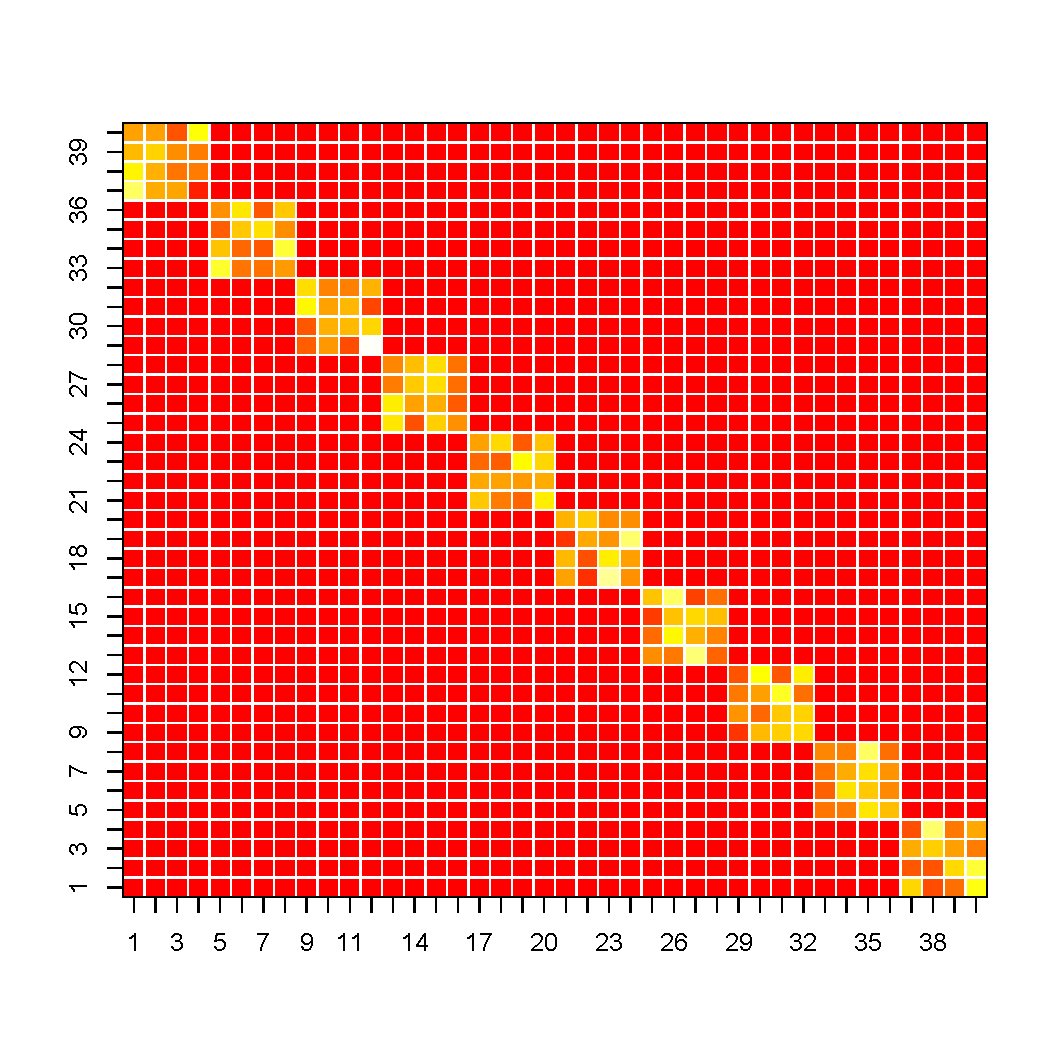
\includegraphics[width=0.6\textwidth]{fig/block_diag/A_gt_10x4.pdf}
% \caption{Ground truth transition matrix for block diagonal
%   experiment.  Yellow indicates high transition probability.
%   40 total states are grouped into 10 groups of 4, with high
%   transition probabilities within a group and low transition
%   probabilities between groups. 
%   \label{fig:block-diag-gt-transition}}
% \end{figure}

% Each of the forty states was associated with a mean in a
% two-dimensional observation space.  However, unlike in the experiments
% discussed in Chapters \ref{chapter:cocktail-party} and
% \ref{chapter:REDD}, there was no relationship between proximity in
% transition space and proximity in emission space: the means for the
% twelve states were drawn independently from a bivariate $\Norm{0}{\sigma^2 I}$
% distribution, where $\sigma^2 = 2$ in this data.

% A sequence of 1000 state labels was generated from the HMM. 
% At each time step, an observation was drawn from a bivariate
% $\Norm{\mu_{z_t}}{I}$ distribution.  Observations color coded by ground
% truth state are shown in Fig. \ref{fig:block-diagonal-gt-observations}.

% \begin{figure}
% \centering
% 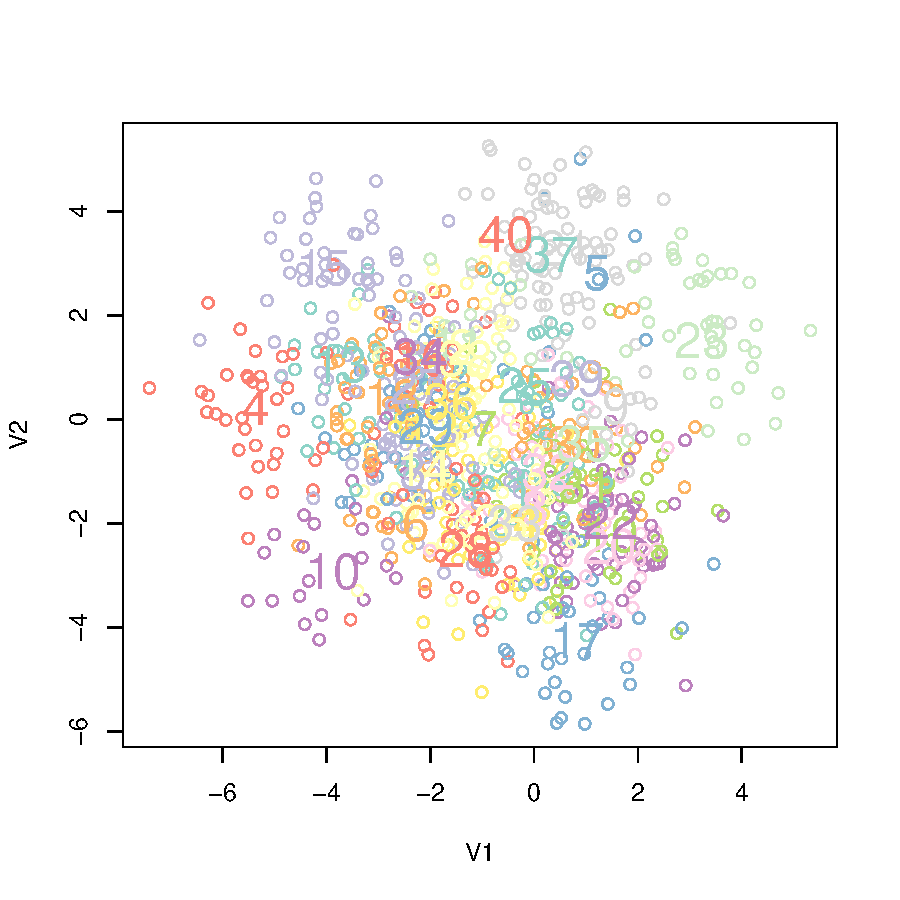
\includegraphics[width=0.6\textwidth]{fig/block_diag/10x4_gty.pdf}
% \caption{Observations generated from the near-block-diagonal HMM,
%   color-coded by ground truth state label.
%   \label{fig:block-diagonal-gt-observations}}
% \end{figure}

% Since the HaMMLeT model infers a latent location for each state, and
% since the latent state locations impact the transition matrix by
% promoting transitions between nearby states and suppressing
% transitions between far away states, it is predicted that the HaMMLeT
% model will locate states in the same superstate near each other, and
% so we should expect to see a ``clustering'' of states into three
% distinct groups based on their $\eta_j$ vectors.  This clustering
% ability should allow HaMMLeT to more efficiently learn the correct
% near-block-diagonal transition matrix as compared to the HDP-HMM 
% with no preference for local transitions.


% \subsection{Results}

% Because there is nothing in the data or the model to provide an
% ordering of the latent states, it is not useful to compare the latent
% state sequences themselves, as there are many possible alignments between ground truth and
% inferred state labels is not specified.   
% Instead, to evaluate the performance of HaMMLeT versus the ordinary HDP-HMM,
% each model's calculated marginal log likelihood was computed based on
% both the training data set used during inference, and on a held-out
% test set (of the same length as the training set: 1000 observations).  
% At each Gibbs iteration, the marginal log likelihood was
% computed by fixing the transition matrix and emission parameters, and
% integrating out the state sequence using the forward message passing
% algorithm.  For each model (HaMMLeT and the ordinary HDP-HMM), ten 
% Gibbs runs of 10,000 iterations each were completed on the data.  The
% results by iteration are shown in
% Fig. \ref{fig:block-diag-likelihoods}.  It is also worth examining the inferred
% transition matrices for the two models.
% Fig. \ref{fig:block-diag-inferred-A} shows ``heatmaps'' of the transition matrices
% sampled at the last iteration of the first run of each of the two
% models (the other runs were similar).

% \begin{figure}
% \begin{minipage}{0.45\textwidth}
% 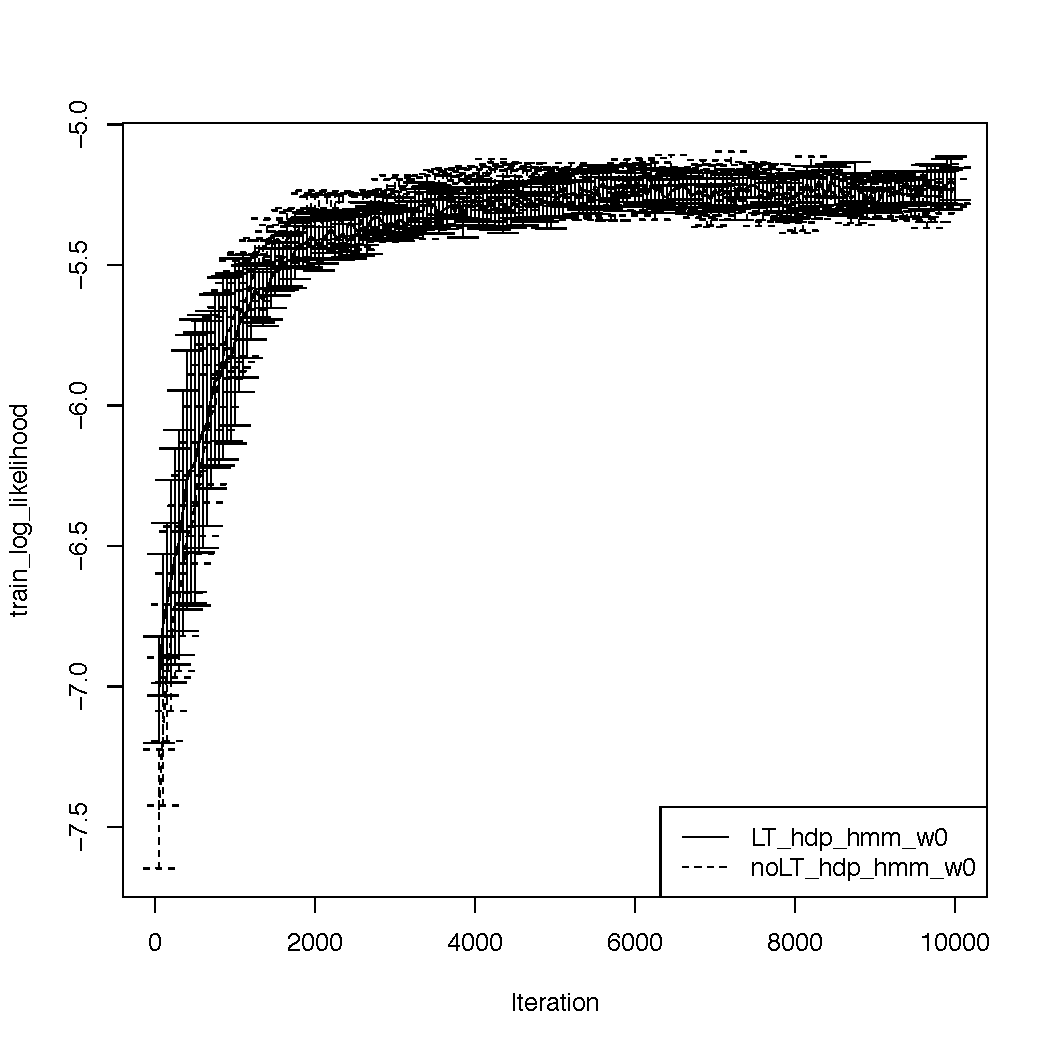
\includegraphics[width=\textwidth]{fig/block_diag/train_log_likelihood}
% \end{minipage}
% \label{fig:block-diag-inferred-A}
% \hspace{0.1in}
% \begin{minipage}{0.45\textwidth}
% 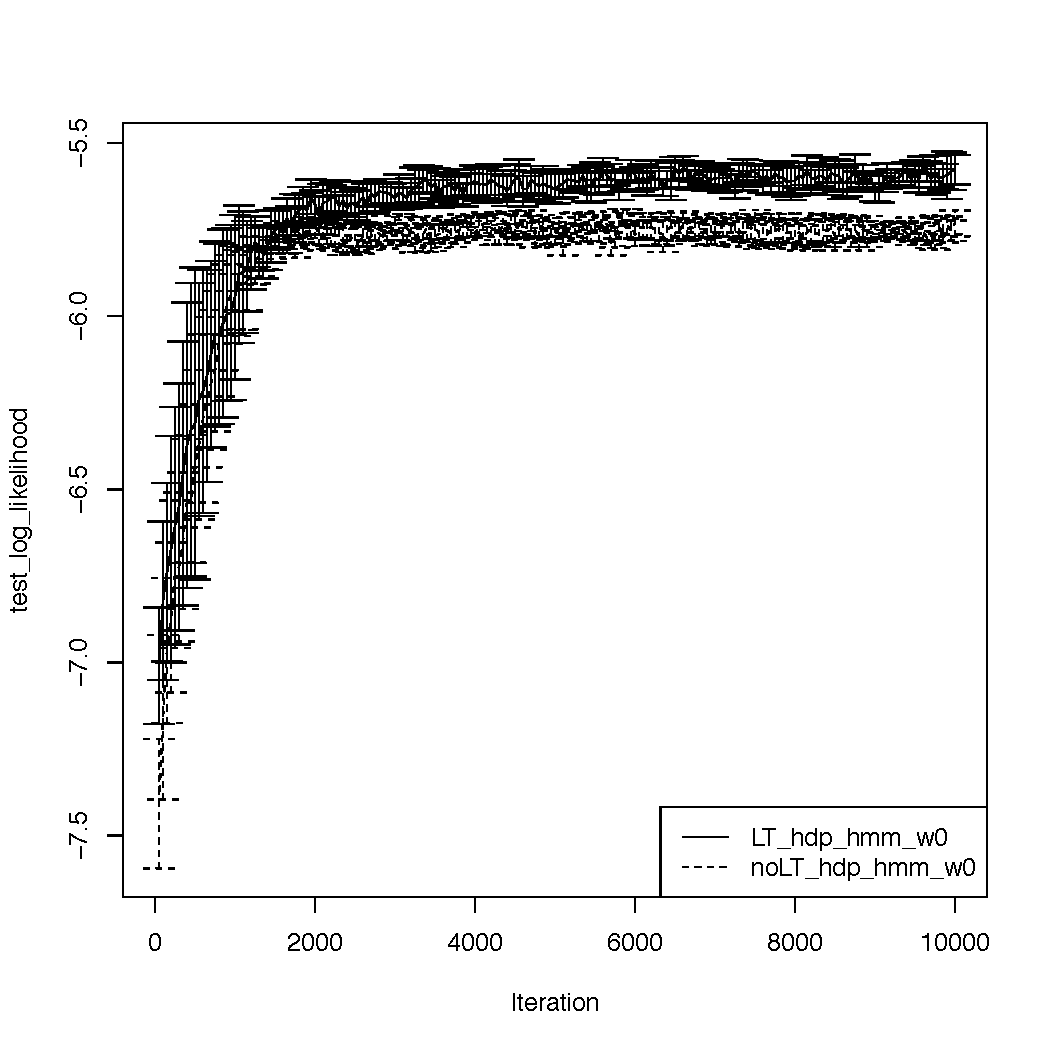
\includegraphics[width=\textwidth]{fig/block_diag/test_log_likelihood}
% \end{minipage}
% \caption{Left: Log likelihood on the near-block-diagonal HMM training set by Gibbs iteration
%   (marginalizing out state sequence) for LT and no LT (HDP-HMM)
%   models.  Right: Log likelihood on a held out test set generated by
%   the same HMM.  In all cases, the trend line represents the mean log
%   likelihood per iteration over the 10 Gibbs runs, and error bars represent 99\% confidence
%   intervals.  
%   \label{fig:block-diag-likelihoods}}
% \end{figure}

% \begin{figure}
%   \centering
%   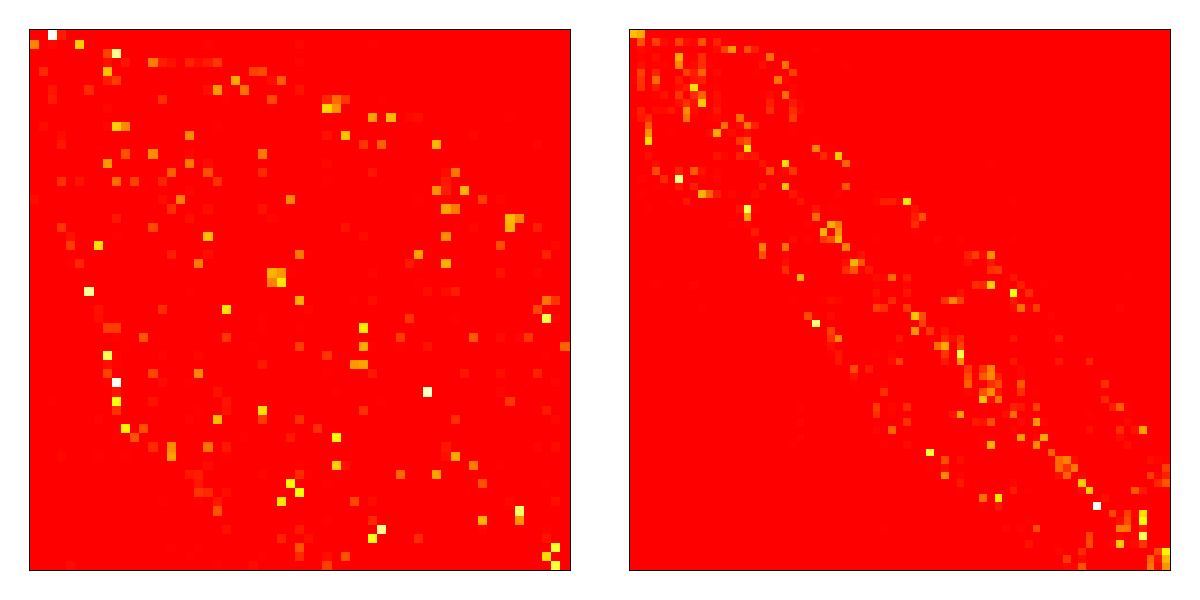
\includegraphics[width=\textwidth]{fig/block_diag/A01.pdf}\\
%   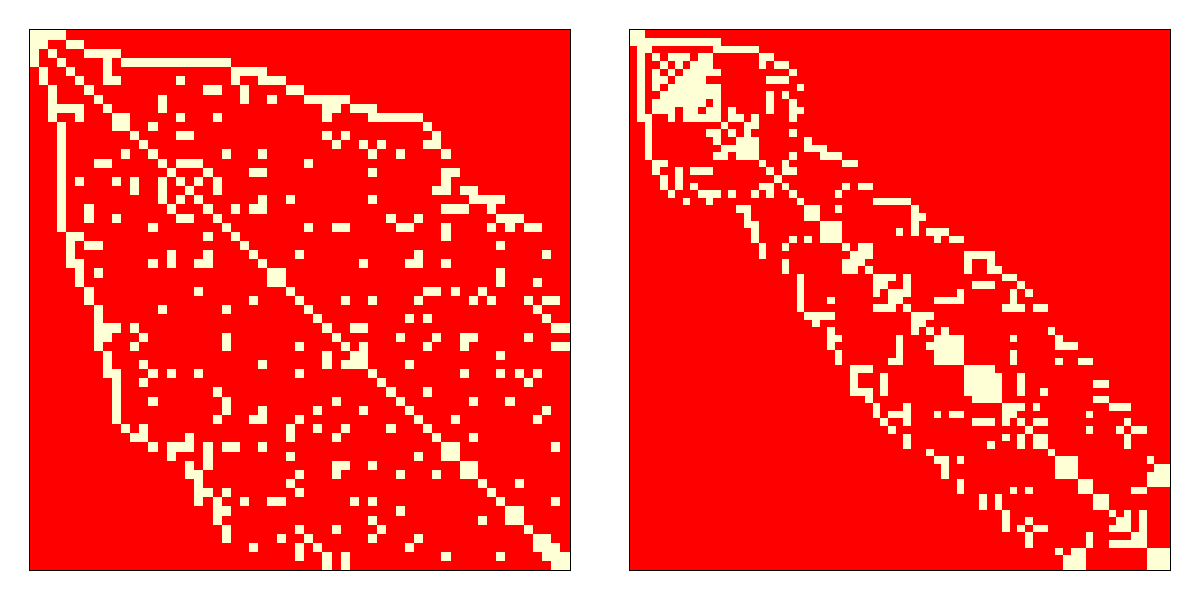
\includegraphics[width=\textwidth]{fig/block_diag/A01-binary.pdf}
%   \caption{Top: Inferred transition matrices for the ordinary HDP-HMM model
%     (left) and the HDP-HMM-LT (right) on the synthetic data from the
%     near-block-diagonal 40 state HMM.  Yellow corresponds to high
%     probability. Bottom: The average of the transition matrices and
%     their transposes, thresholded.   The light
%     color corresponds to average transition probabilities in excess of $2 /
%     J_{used}$, where $J_{used}$ is the number of distinct states actually
%     visited at some point by the inferred state sequence. The
%     LT model is again on the right. In both the top and bottom, only states that
%     actually occur in the inferred sequence are shown, and the order of the
%     states have been permuted using the Reverse Cuthill-McKee
%     algorithm \cite{cuthill1969reducing} to minimize the ``bandwidth'' of the transition matrices
%     (the number of diagonals with high probability). \label{fig:block-diag-inferred-A}}
% \end{figure}

% The two models performed equally well on the training set, as measured
% by marginal likelihood, but the LT model had a small but
% consistent edge on the held out data, suggesting that it is doing less
% overfitting, and recovering a more faithful approximation to the
% generating process.  This conclusion is corroborated by the transition
% matrices: while neither model recovers a perfect block-diagonal
% structure, there is a clear difference between the ``bandwidth'' of the
% two models' inferred matrices, with the LT model producing a more
% compact matrix which is closer to the true ``septa-diagonal''
% structure of the 10 by 4 ground truth matrix.

\section{Discovering Chord Equivalence Classes in Tonal Music}
\label{sec:disc-chord-equiv}

A real-world test of the separable-similarity form of HaMMLeT comes
from the music domain.  Two datasets were used, one generated from a
an artificial musical grammar, the other based on Bach chorales. 
In both cases, each observation consisted of four musical tones played concurrently, 
constituting a chord, and the sequences between chords followed 
conventions for Western tonal music.  

\subsection{Emission Model}
\label{sec:emission-model}

The emission model used for the music data is Dirichlet-Categorical,
with each state modeled using a categorical distribution over the 120
integer chord symbols, with a symmetric Dirichlet prior on 
the emission distributions.  In the experiments reported here the
concentration parameter was 1.0.

\subsection{Synthetic Data}
\label{sec:data-generation}

\paragraph{Data-Generation}
To create the first dataset, two 500-chord sequences were
generated by the Kulitta generative grammar \cite{quick2014kulitta},
one used as a training set and the other used as a test set.  A score from
an excerpt of the training sequence is in Fig. \ref{fig:music-score}.
The chord sequences were preprocessed for the model by translating
each chord to a single integer value, with each
distinct set of four tones receiving a distinct label.  In total,
throughout the two 500-chord sequences, 120 distinct chords appeared,
13 of which are unique to the test set.
The sparsity of the observed data suggests that a more compact latent
state representation might be useful.  Of interest is whether the models can
discover such a representation, grouping the observed chords into
``equivalence classes''.

\begin{figure}[t]
  \centering
  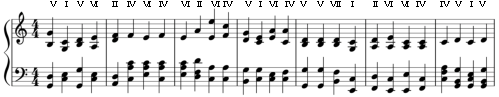
\includegraphics[width=\textwidth]{fig/music/chord1/chords_annotated.pdf}
  \caption{Transcription of a segment of a four-voice chorale produced
    by Kulitta, annotated with chord equivalence classes.  The full
    data sequence was 500 chords long.}
  \label{fig:music-score}
\end{figure}


\paragraph{Results}
In this data there is no ground truth latent state sequence to compare
the results to, so as in the block-diagonal data above, marginal
likelihood on training and test sets is used as a performance metric,
computed at each iteration using forward message-passing.  Results are
in Fig. \ref{fig:music-likelihoods}.  As with the block-diagonal data,
the LT model does not show a likelihood advantage on the training data
(in fact, its marginal likelihood is lower); but the LT model performs 
consistently better at generalizing to the test set.  This suggests
that the more informative prior on the transition matrix 
is helping to extract stable structure, and avoid overfitting the
statistics of the training set.

\begin{figure}[tb]
% \vskip 0.1in
\begin{center}
  \centerline{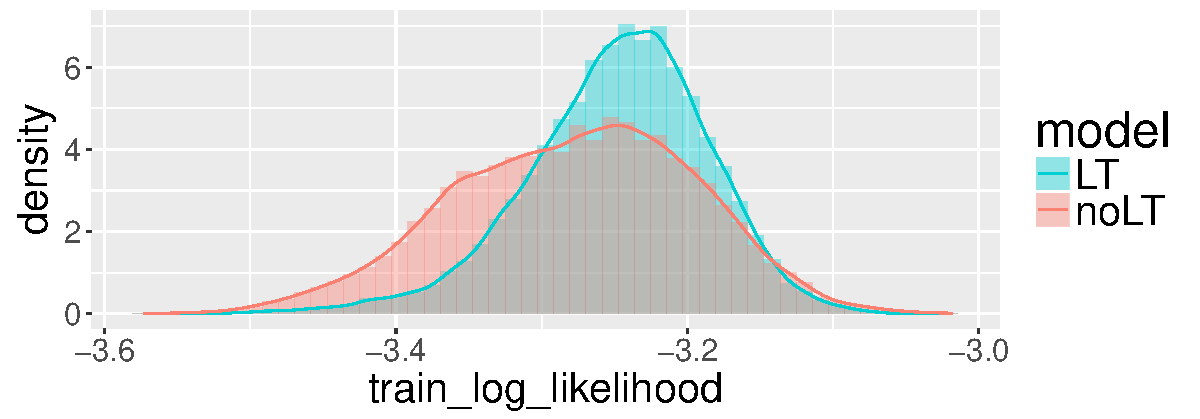
\includegraphics[width = 0.75\columnwidth]{fig/music/chord1/train_log_likelihood_density.pdf}}
  \centerline{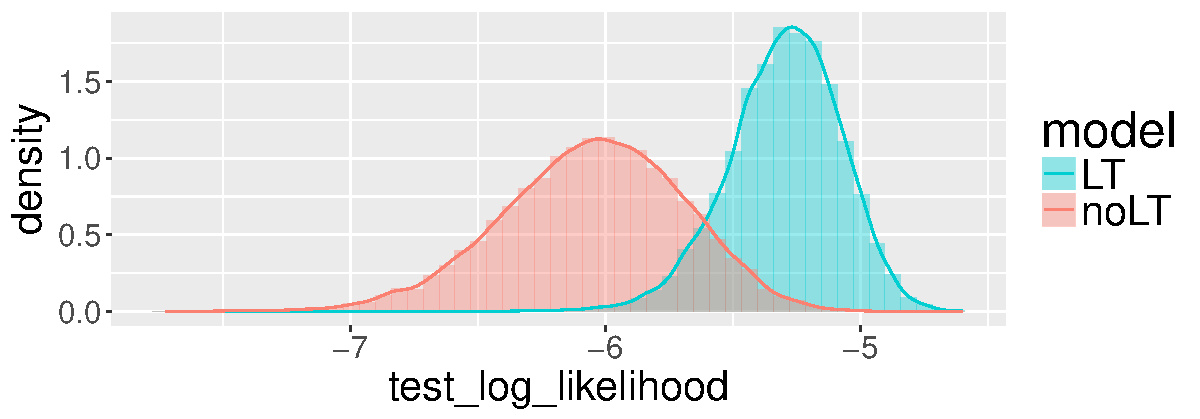
\includegraphics[width = 0.75\columnwidth]{fig/music/chord1/test_log_likelihood_density.pdf}}
  \centerline{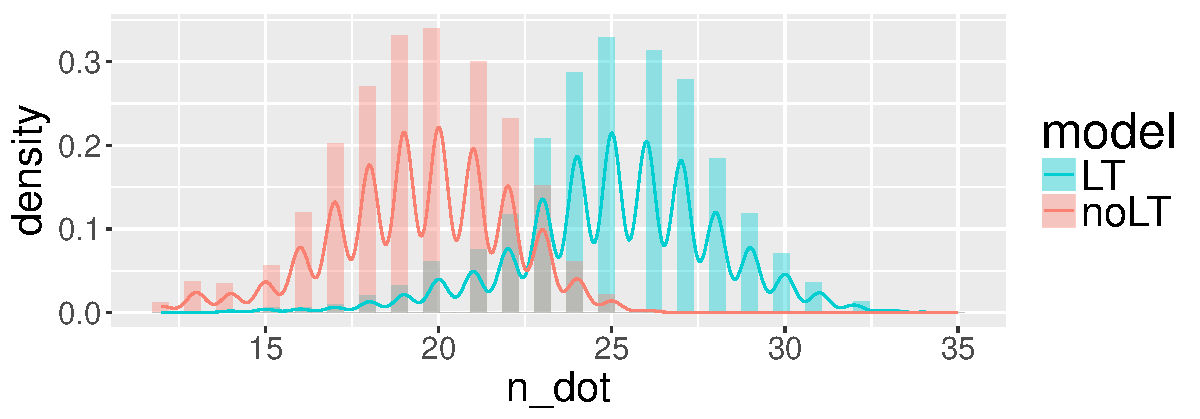
\includegraphics[width = 0.75\columnwidth]{fig/music/chord1/n_dot_density.pdf}}
\caption{Top: Log likelihood on the Kulitta training set by Gibbs iteration
  (marginalizing out state sequence) for four models
  models.  Middle: Log likelihood on a held out test set generated by
  the same Kulitta grammar.  Bottom: the number of occupied
  states in the training data. \label{fig:music-likelihoods}}
\end{center}
% \vskip 0.1in
\end{figure}

It is also of interest to examine the set of latent states discovered
by the two models, and in particular the degree to which the
stochastic map between latent states and produced chords approximates
a one-to-many structure.  The emission distributions for the last
iteration of the first run of each model are shown in
Fig. \ref{fig:music-emissions}.  Notably, the LT model does a better
job of partitioning chord symbols, with fewer instances of a single
chord being generated with relatively high probability in more than
one state, as can be seen by examining how often a column contains
more than one high probability entry (bright squares in the figure).

\begin{figure}[t]
  \centering
  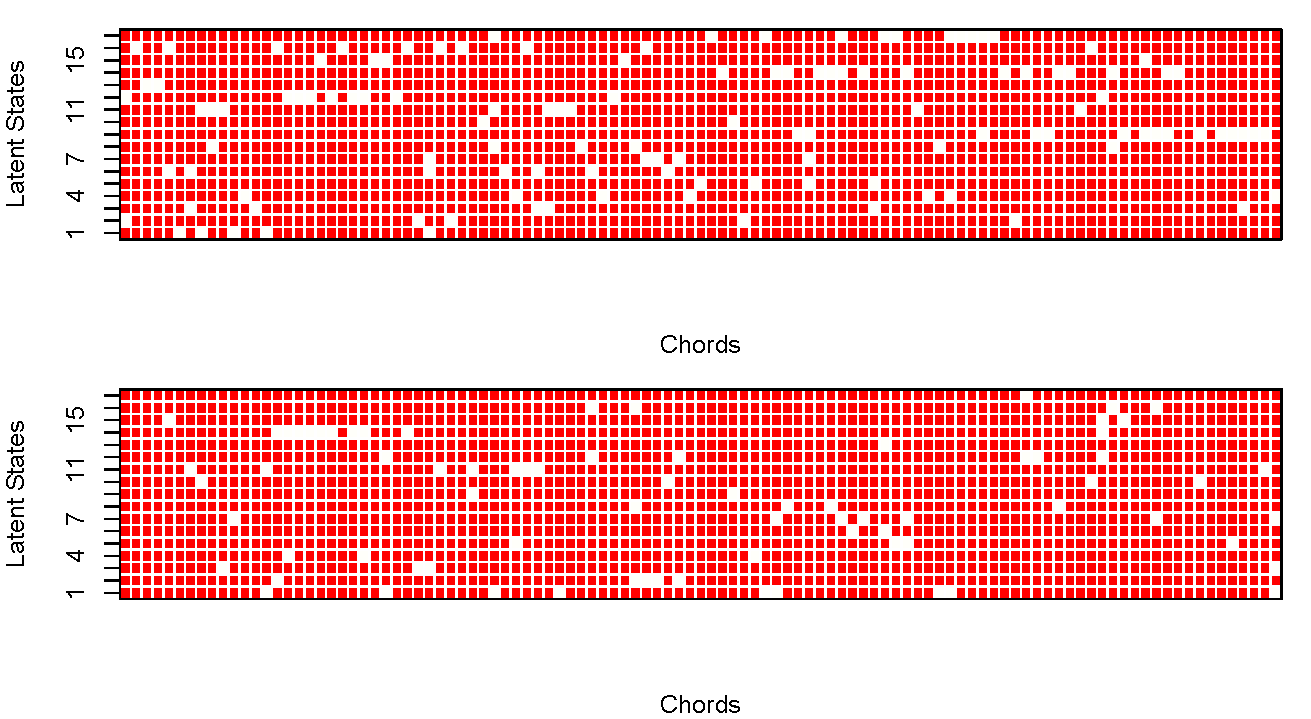
\includegraphics[width=\textwidth]{fig/music/chord1/chord_emissions.pdf}
  \caption{Emission distributions of the states discovered by the
    HDP-HMM (top) and the HDP-HMM-LT (bottom). Rows correspond to
    latent states actually visited during either the training or test
    sequence; columns represent the distinct chord symbols emitted.
    Emission probabilities are thresholded at 3 times the relative
    frequency of a chord in the corpus, so that bright spots
    correspond to a higher-than-average probability of emitting a
    particular chord, irrespective of how common or rare the chord is.
    \label{fig:music-emissions}}
\end{figure}

\subsection{Bach Chorales}

A second music experiment used the same model but evaluated it using 
a real, and much larger dataset, namely a corpus of 217 four-voice
major key chorales by J.S. Bach from
music21\footnote{\url{http://web.mit.edu/music21}}.

\paragraph{Data}
Two-hundred chorales from the corpus were randomly selected
as a training set, with the other 17 used as a test set to evaluate
surprisal (marginal log likelihood per observation) by the trained
models.  All chorales were transposed to C-major, and each
distinct four-voice chord (with voices ordered) 
was encoded as a single integer.  In total
there were 3307 distinct chord types and 20401 chord tokens in the 217
chorales, with 3165 types and 18818 tokens in the 200 training
chorales, and 143 chord types that were unique to the test set.

Since the chords were encoded as integers, the emission distribution
for each state is $\Cat{\btheta_j}$.  We use a 3307-dimensional 
symmetric Dirichlet prior for each $\btheta_j$, resulting in conjugate 
updates to $\btheta$ conditioned on the latent state sequence, $\bz$.

The prior on each $\ell$ was bivariate
$\Norm{0}{\mathbf{I}}$, and the similarity funciton was squared exponential
based on Euclidean distance: $\phi_{jj} =
\exp\{-\lambda d_2(\ell_j, \ell_{j'})^2\}$ where $d_2$ is Euclidean
distance.  % Since the latent
% states are now continuous, we use a Hamiltonian Monte Carlo (HMC) update
% \cite{duane1987hybrid, neal2011mcmc} to update of the $\bell_j$
% simultaneously, conditioned on $\bz$ and $\bpi$.  
% HMC is a variation on Metropolis-Hastings
% algorithm which is designed to more efficiently explore a
% high-dimensional continuous distribution by adopting a proposal
% distribution which incorporates an auxiliary ``momentum'' variable to
% make it more likely that proposals will go in useful directions and
% improve mixing compared to naive movement.  The HMC update requires
% the gradient of the log (conditional) posterior.  The relevant prior
% and likelihood are
% \begin{align}
% \begin{split}
%   p(\bell_j) &\propto -\frac{1}{2} \norm{\ell_j}^2 \\
%   p(\bz, \bu, \bQ \given \bell) &\propto \prod_j \prod_{j'}
%   \phi_{jj'}^{n_{jj'}}(1 - \phi_{jj'})^{q_{jj'}}.
% \end{split}
% \end{align}
% The coordinate of the gradient of the log likelihood corresponding to
% dimension $d$ in state $j$ is
% \begin{equation*}
%   \frac{\partial \log L}{\partial \bell_{jd}} = -\lambda
%   \sum_{(j,j'):j \neq j'} (\ell_{jd} - \ell_{j'd}) \left(n_{jj'} - q_{jj'} \frac{\phi_{jj'}}{1 - \phi_{jj'}}\right)
% \end{equation*}

\paragraph{Results}
\label{sec:results}

Four models: HDP-HMM-LT, Sticky-HDP-HMM-LT, HDP-HMM and
Sticky-HDP-HMM, were evaluated on the Bach data using 5 Gibbs chains
running for 10,000 iterations 
each on the 200 training chorales, which were modeled as conditionally independent
of one another.  Every 50th iteration, the
marginal log likelihood was calculated on the 17 test chorales
(integrating out $\bz$).  The distributions of the training and test log
likelihoods are in Fig. \ref{fig:bach-metric}.  Although the LT
model does not achieve as close a fit to the training data, its
generalization performance is better, suggesting that the HDP-HMM
without the local transition property is overfitting.  In fact, the
vanilla HDP-HMM and Sticky HDP-HMM are maxing out their state
allowances at 200, whereas the LT models average closer to 150 state.
It is perhaps counterintuitive that the LT property would protect against
overfitting, as it has more free parameters.  However,
the similarity bias induces greater sharing of information across
parameters, as in a hierarchical model: instead of each entry
$\pi_{jj'}$ being informed only by transitions from j to j', it is 
informed to some extent by *all* transitions, as all transitions
inform the similarity structure.

\begin{figure}[tb]
% \vskip 0.1in
\begin{center}
  % \centerline{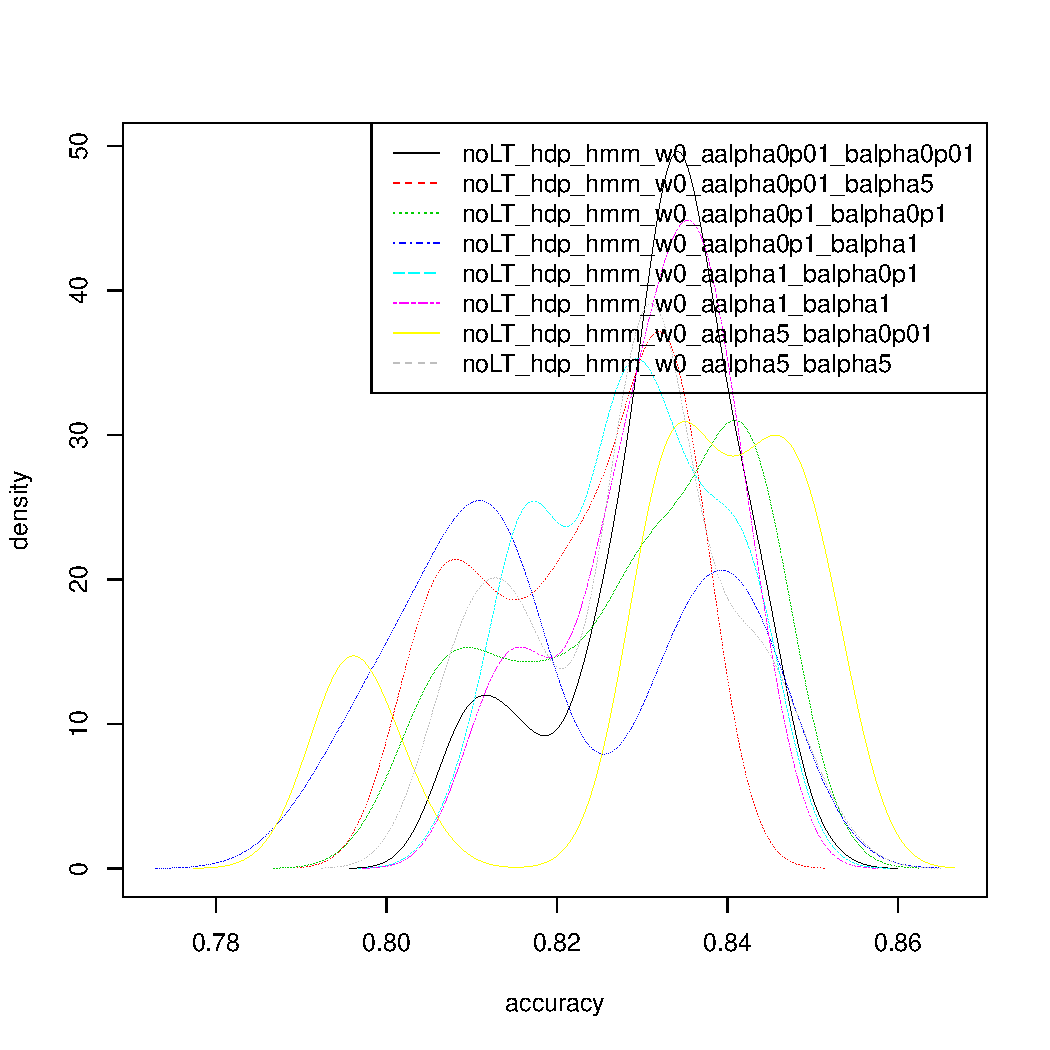
\includegraphics[width = \columnwidth]{fig/cocktail/accuracy_density.pdf}}
  \centerline{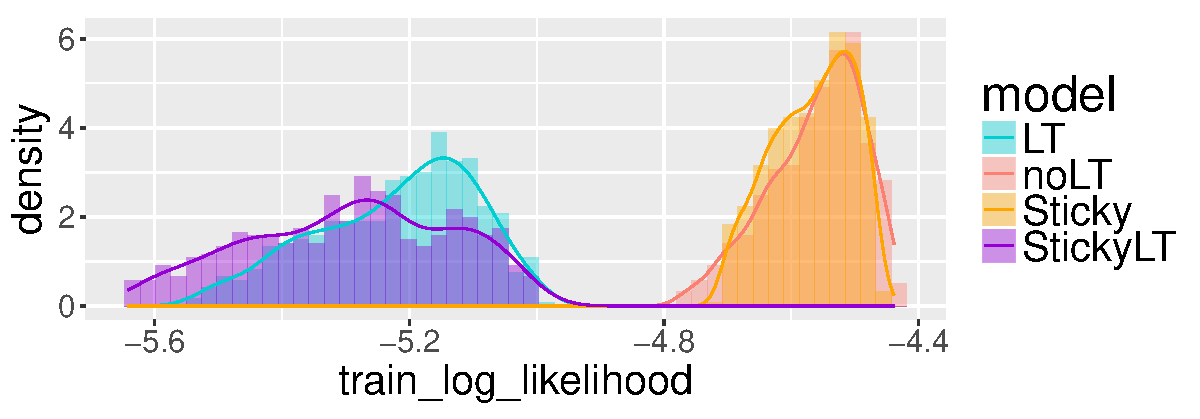
\includegraphics[width = 0.75\columnwidth]{fig/music/bach/lambda5/train_log_likelihood_density.pdf}}
  \centerline{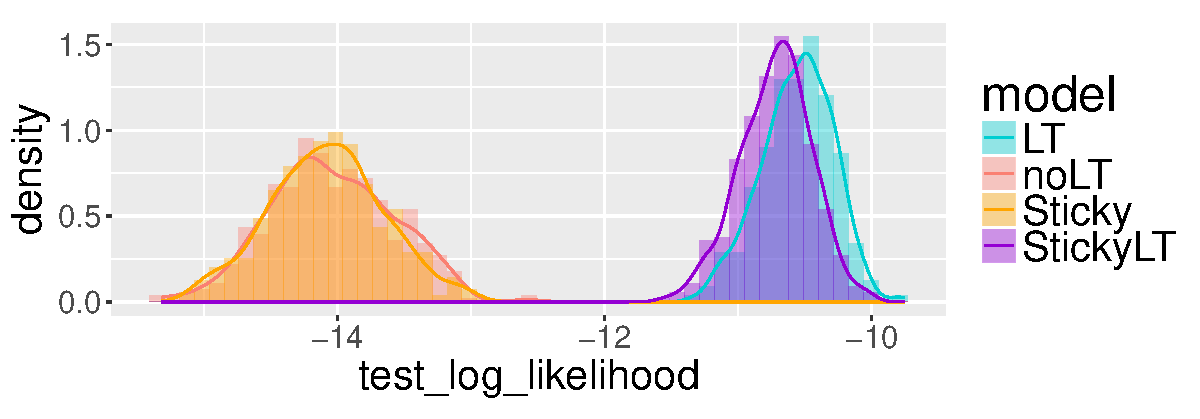
\includegraphics[width = 0.75\columnwidth]{fig/music/bach/lambda5/test_log_likelihood_density.pdf}}
  \centerline{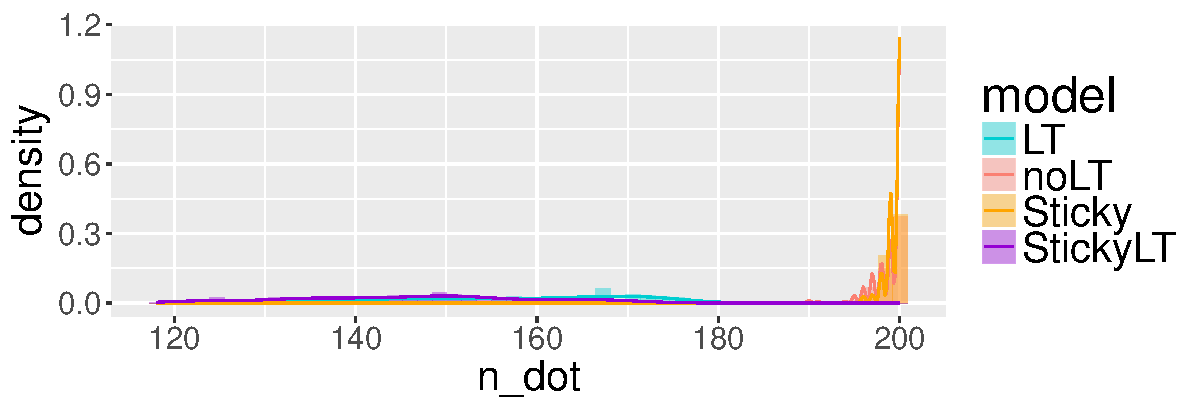
\includegraphics[width = 0.75\columnwidth]{fig/music/bach/lambda5/n_dot_density.pdf}}
  % \centerline{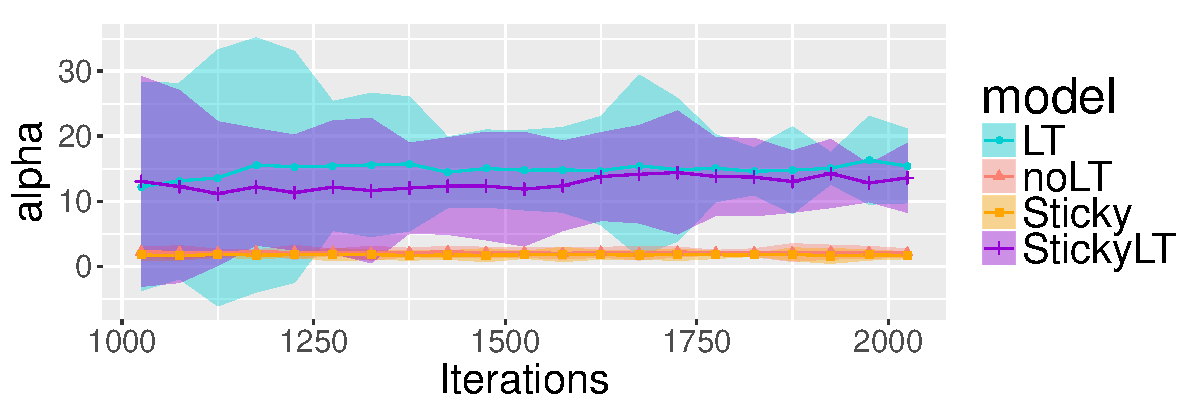
\includegraphics[width = \columnwidth]{fig/bach/alpha.pdf}}
\caption{Top and Middle: Training set and test set log marginal likelihoods for Bach
  chorale data on the four HDP-based models: HDP-HMM-LT, HDP-HMM,
  Sticky HMM, and Sticky HDP-HMM-LT.  Bottom: Number of latent states
  occupied in the training set by each model. \label{fig:bach-metric}
}
\end{center}
% \vskip 0.1in
\end{figure}
